\documentclass[a4paper,11pt]{article}
\usepackage[T1]{fontenc}
\usepackage[utf8]{inputenc}
\usepackage{lmodern}
\usepackage{upgreek}
\usepackage{amsmath}
\usepackage{mathabx}
\usepackage{MnSymbol}
\usepackage{wasysym}
\usepackage{booktabs}
\usepackage{graphicx}
\usepackage[]{algorithm2e}
\usepackage{hyperref}
\usepackage{tikz}

\title{Programovací jazyk SVGER}

\begin{document}

\maketitle

\newpage
\tableofcontents

\newpage
\section{Gramatiky}
V této sekci se nachází popis jednotlivých gramatik, které jsou zpracovány lexikálním analyzátorem.

\subsection{Identifikátory}
Identifikátor začíná na kterýkoliv znak z množiny $z = \{a..z, A..Z, +, -, /, *, <\}$
a pokračuje v libovonlném znaku z množiny $m = z \bigcup \{0..9\}$ 
\linebreak

$G_{identifikatory}$(\{S, A, B\}, \{z, m\}, P, S)
$$S \rightarrow zA | z$$
$$A \rightarrow mA | m$$

\subsection{Čísla}
$G_{cisla}$(\{S, B, C\}, \{d, .\}, P, S)
$$S \rightarrow dB | d$$
$$B \rightarrow dB | d | .C$$
$$C \rightarrow dC | d$$



\subsection{Řetězce}
Řetězce začínají a končí na znak ". V samotném řetězci se pak může nacházet jakýkýkoliv znak před kterým se nachází $\backslash$ nebo cokoliv v množině $\blacksquare$, která reprezentuje všechny tisknutelné znaky, které nejsou $\backslash$ nebo ".

$G_{retezce}$(\{S, D, E\}, \{$\backslash, ", \blacksquare$\}, P, S)
$$S \rightarrow "D$$
$$D \rightarrow " | \backslash E | \blacksquare E$$
$$E \rightarrow "D | \backslash D | \blacksquare D$$

\subsection{Závorky}
Závorky hrají v lispu důležitou roli. Rozhodl jsem se, že pro jednoduchost bude jazyk podporovat jen \textquotedblleft kulaté \textquotedblright závorky
$G_{zavorky}$(\{S\}, \{(, )\}, P, S)

$$S \rightarrow (|)$$

\subsection{Gramatika bílých znaků}
Je gramatika popisující všechny bílé znaky $G_{bileznaky}$(\{S\}, \{$\dlsh | \mapsto | \sqcup$\}, P, S)
$$S \rightarrow  \dlsh S | \mapsto S | \sqcup S$$

\subsection{Komentáře}
Jazyk má jednoduché komentáře začínající na ; a končící novým řádkem $G_{komentare}$(\{S, F\}, \{$\dlsh$, ;, $\Square$\}, P, S)

$$S \rightarrow ;F$$
$$F \rightarrow \Square F | \dlsh S$$

\subsection{Symboly pro expanzi parserem}
$G_{expanze}$(\{S, G\}, \{ $\boxplus$, \# \})

$$S \rightarrow \#G$$
$$G \rightarrow \boxplus G | \boxplus$$

Kde $\boxplus$ je množina všech nebilých znaků včetně \#. 

\subsection{Speciální znaky}
$G_{specialni}$(\{S\}, \{, , ` , ', '@', \textasciitilde{} \})

$$S \rightarrow  , | ` | ' | @ | \textasciitilde{}$$

\subsection{Logické hodnoty}
Logická hodnota může být buď PRAVDA nebo NEPRAVDA tedy:
$G_{logicke}$(\{S, H, I, J, K, L, M, O\}, \{P, R, A, V, D, A, N, E\})

$$S \rightarrow N H | P J$$
$$H \rightarrow E I$$
$$I \rightarrow P J$$ 
$$J \rightarrow R K$$
$$K \rightarrow A L$$
$$L \rightarrow V M$$
$$M \rightarrow D O$$
$$O \rightarrow A$$

\section{Stavový automat}
Nyní je třeba z předem definované gramatiky spojit a převést na automat. Pokud tento automat nebude deterministický je třeba jej determinizovat.

Samotný jazyk se skládá z jazyku oddělovačů (komentáře, bílé znaky) $L_{od} = G_{komentare} \bigcup G_{bileznaky}$ a jazyku významových tokenů. 

$$L_{vt} = L_{identifikatory} \bigcup L_{cisla} \bigcup L_{retezce} \bigcup L_{zavorky}$$
Celý jazyk pak lze zapsat tímto způsobem 
$$L = (L^{*}_{od}.L_{vt})^{*}.L^{*}_{od}$$
Po spojení nám vzniká gramatika
 
%%% Gramatika
$G_{vt}$(\{S, $S_{identifikatory}$, $S_{cisla}$, $S_{retezce}$, $S_{zavorky}$, A, B, C, D, E, F, G\}, \{d, z, m, (, ), $\backslash$ \}, P, S), která reprezentuje významové tokeny 

$$S \rightarrow S_{identifikatory} | S_{cisla} | S_{retezce} | S_{zavorky} | S_{od}$$

kde neterminál $S_{od}$ je definovaný v gramatice oddělovačů $G_{od}$(\{S, A\}, \{$\mapsto$, $\sqcup$, $\dlsh$, ;\}, P, S)

$$S \rightarrow \dlsh | \mapsto | \sqcup | ;A | \Square$$
$$A \rightarrow \Square A | ;A | \dlsh $$

Po spojení gramatik a odstranění jednoduchých pravidel dostaváme gramatiku
$G_{finalni}$(\{$S_{od}$\}, \{$\mapsto$, $\sqcup$, $\dlsh$, ;, $\Square$, $\backslash$, $\blacksquare$, ", d, ., z, m, (, )\}, P, S)
$$S \rightarrow zA | z | dB | d | "D | ;F | \dlsh S | \mapsto S | \sqcup S | ( | )$$
$$A \rightarrow mA | m$$
$$B \rightarrow dB | d | .C$$
$$C \rightarrow dC | d$$
$$D \rightarrow " | \backslash E | \blacksquare D$$
$$E \rightarrow "D | \backslash D | \blacksquare D$$
$$F \rightarrow \Square F | \dlsh S$$
\newpage

\begin{table}[]
\centering
\resizebox{\textwidth}{!}{%
\begin{tabular}{@{}lllllllllllllll@{}}
\toprule
$\delta$& d & z & m & ( & ) & $\blacksquare$ & $\Square$ & $\backslash$ & ; & . & " & $\dlsh$ & $\mapsto$ & $\sqcup$   \\ \midrule
$Q_{S}$ & $Q_{B\hat{F}}$ & $Q_{A\hat{F}}$ & - & $Q_{\hat{F}}$ & $Q_{\hat{F}}$ & - & - & - & $Q_{F}$ & - & $Q_{D}$ & $Q_{S}$ & $Q_{S}$ & $Q_{S}$ \\
$Q_{C}$ & $Q_{C\hat{F}}$ & - & - & - & - & - & - & - & - & - & - & - & - & - \\
$Q_{D}$ & - & - & - & - & - & $Q_{D}$ & - & $Q_{E}$ & - & - & $Q_{\hat{F}}$ & - & - & - \\
$Q_{E}$ & - & - & - & - & - & $Q_{D}$ & - & $Q_{D}$ & - & - & $Q_{D}$ & - & - & - \\
$Q_{F}$ & - & - & - & - & - & - & $Q_{F}$ & - & - & - & - & $Q_{S}$ & - & - \\
$Q_{\hat{F}}$ & - & - & - & - & - & - & - & - & - & - & - & - & - & - \\
$Q_{A\hat{F}}$ & - & - & $Q_{A\hat{F}}$ & - & - & - & - & - & - & - & - & - & - & - \\
$Q_{B\hat{F}}$ & $Q_{B\hat{F}}$ & - & - & - & - & - & - & - & - & $Q_{C}$ & - & - & - & - \\
$Q_{C\hat{F}}$ & $Q_{C\hat{F}}$ & - & - & - & - & - & - & - & - & - & - & - & - & - \\ \bottomrule
\end{tabular}%
}
\caption{Determinizovaný automat}
\label{f}
\end{table}

\begin{center}
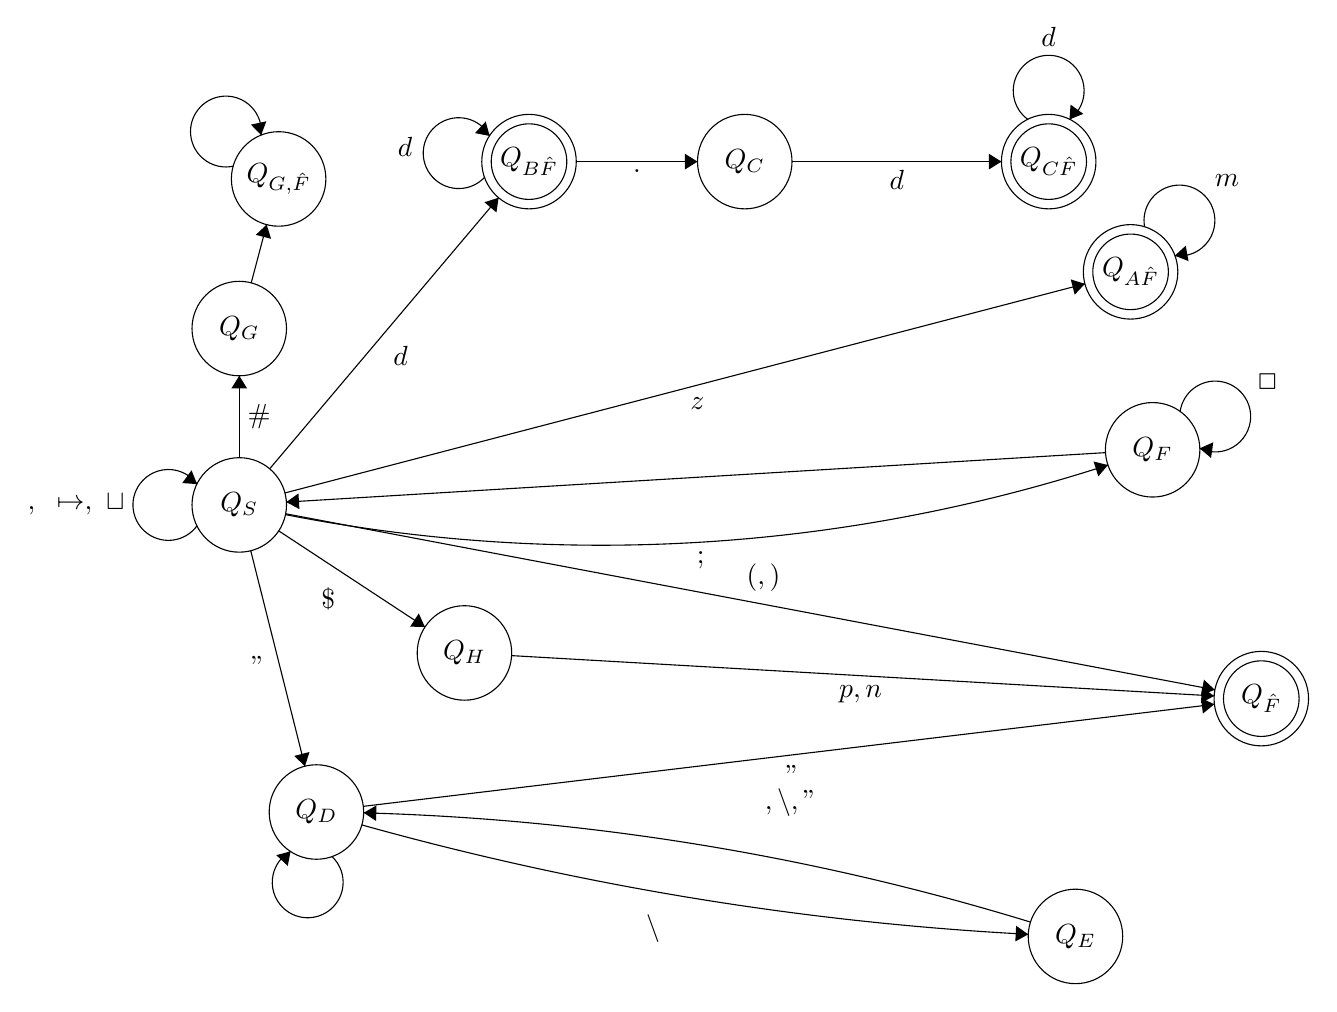
\begin{tikzpicture}[scale=0.2]
\tikzstyle{every node}+=[inner sep=0pt]
\draw [black] (8,-28.2) circle (3);
\draw (8,-28.2) node {$Q_{S}$};
\draw [black] (26.4,-6.4) circle (3);
\draw (26.4,-6.4) node {$Q_{B\hat{F}}$};
\draw [black] (26.4,-6.4) circle (2.4);
\draw [black] (64.6,-13.4) circle (3);
\draw (64.6,-13.4) node {$Q_{A\hat{F}}$};
\draw [black] (64.6,-13.4) circle (2.4);
\draw [black] (72.9,-40.5) circle (3);
\draw (72.9,-40.5) node {$Q_{\hat{F}}$};
\draw [black] (72.9,-40.5) circle (2.4);
\draw [black] (59.4,-6.4) circle (3);
\draw (59.4,-6.4) node {$Q_{C\hat{F}}$};
\draw [black] (59.4,-6.4) circle (2.4);
\draw [black] (12.9,-47.7) circle (3);
\draw (12.9,-47.7) node {$Q_{D}$};
\draw [black] (66,-24.7) circle (3);
\draw (66,-24.7) node {$Q_{F}$};
\draw [black] (61.1,-55.6) circle (3);
\draw (61.1,-55.6) node {$Q_{E}$};
\draw [black] (40.1,-6.4) circle (3);
\draw (40.1,-6.4) node {$Q_{C}$};
\draw [black] (22.3,-37.6) circle (3);
\draw (22.3,-37.6) node {$Q_{H}$};
\draw [black] (8,-17) circle (3);
\draw (8,-17) node {$Q_{G}$};
\draw [black] (10.5,-7.5) circle (3);
\draw (10.5,-7.5) node {$Q_{G,\hat{F}}$};
\draw [black] (9.93,-25.91) -- (24.47,-8.69);
\fill [black] (24.47,-8.69) -- (23.57,-8.98) -- (24.33,-9.63);
\draw (17.75,-18.74) node [right] {$d$};
\draw [black] (10.9,-27.44) -- (61.7,-14.16);
\fill [black] (61.7,-14.16) -- (60.8,-13.88) -- (61.05,-14.85);
\draw (37.09,-21.37) node [below] {$z$};
\draw [black] (10.95,-28.76) -- (69.95,-39.94);
\fill [black] (69.95,-39.94) -- (69.26,-39.3) -- (69.07,-40.28);
\draw (41.29,-33.71) node [above] {$(,)$};
\draw [black] (65.49,-10.547) arc (190.39718:-97.60282:2.25);
\draw (70.72,-8.03) node [above] {$m$};
\fill [black] (67.41,-12.37) -- (68.28,-12.72) -- (68.1,-11.74);
\draw [black] (58.077,-3.72) arc (234:-54:2.25);
\draw (59.4,0.85) node [above] {$d$};
\fill [black] (60.72,-3.72) -- (61.6,-3.37) -- (60.79,-2.78);
\draw [black] (8.73,-31.11) -- (12.17,-44.79);
\fill [black] (12.17,-44.79) -- (12.46,-43.89) -- (11.49,-44.14);
\draw (9.69,-38.41) node [left] {$"$};
\draw [black] (63.16,-25.667) arc (-72.01092:-101.08244:104.23);
\fill [black] (63.16,-25.67) -- (62.25,-25.44) -- (62.55,-26.39);
\draw (37.31,-31.12) node [below] {$;$};
\draw [black] (58.103,-55.466) arc (-93.00582:-105.61026:195.334);
\fill [black] (58.1,-55.47) -- (57.33,-54.92) -- (57.28,-55.92);
\draw (34.28,-54.21) node [below] {$\backslash$};
\draw [black] (15.88,-47.34) -- (69.92,-40.86);
\fill [black] (69.92,-40.86) -- (69.07,-40.46) -- (69.19,-41.45);
\draw (43.15,-44.68) node [below] {$"$};
\draw [black] (15.899,-47.753) arc (88.44043:72.94349:159.117);
\fill [black] (15.9,-47.75) -- (16.69,-48.27) -- (16.71,-47.28);
\draw (43.03,-48.03) node [above] {$\blacksquare,\backslash,"$};
\draw [black] (67.745,-22.274) arc (172.01431:-115.98569:2.25);
\draw (72.64,-20.37) node [right] {$\Square$};
\fill [black] (68.99,-24.61) -- (69.71,-25.22) -- (69.85,-24.22);
\draw [black] (5.32,-29.523) arc (-36:-324:2.25);
\draw (0.75,-28.2) node [left] {$\dlsh,\mbox{ }\mapsto,\mbox{ }\sqcup$};
\fill [black] (5.32,-26.88) -- (4.97,-26) -- (4.38,-26.81);
\draw [black] (63.01,-24.88) -- (10.99,-28.02);
\fill [black] (10.99,-28.02) -- (11.82,-28.47) -- (11.76,-27.47);
\draw (36.78,-25.79) node [above] {$\dlsh$};
\draw [black] (13.882,-50.522) arc (46.9079:-241.0921:2.25);
\draw (10.12,-55.53) node [below] {$\blacksquare$};
\fill [black] (11.26,-50.2) -- (10.35,-50.44) -- (11.08,-51.12);
\draw [black] (23.581,-7.392) arc (317.11154:29.11154:2.25);
\draw (19.03,-5.47) node [left] {$d$};
\fill [black] (23.9,-4.77) -- (23.65,-3.85) -- (22.97,-4.59);
\draw [black] (29.4,-6.4) -- (37.1,-6.4);
\fill [black] (37.1,-6.4) -- (36.3,-5.9) -- (36.3,-6.9);
\draw (33.25,-6.9) node [below] {$.$};
\draw [black] (43.1,-6.4) -- (56.4,-6.4);
\fill [black] (56.4,-6.4) -- (55.6,-5.9) -- (55.6,-6.9);
\draw (49.75,-6.9) node [below] {$d$};
\draw [black] (10.51,-29.85) -- (19.79,-35.95);
\fill [black] (19.79,-35.95) -- (19.4,-35.09) -- (18.85,-35.93);
\draw (13.65,-33.4) node [below] {$\$$};
\draw [black] (25.3,-37.77) -- (69.9,-40.33);
\fill [black] (69.9,-40.33) -- (69.13,-39.78) -- (69.08,-40.78);
\draw (47.46,-39.66) node [below] {$p,n$};
\draw [black] (8,-25.2) -- (8,-20);
\fill [black] (8,-20) -- (7.5,-20.8) -- (8.5,-20.8);
\draw (8.5,-22.6) node [right] {$\#$};
\draw [black] (8.76,-14.1) -- (9.74,-10.4);
\fill [black] (9.74,-10.4) -- (9.05,-11.05) -- (10.02,-11.3);
\draw (10.01,-12.75) node [right] {$\boxplus$};
\draw [black] (7.623,-6.69) arc (282.01279:-5.98721:2.25);
\draw (4.94,-1.53) node [left] {$\boxplus$};
\fill [black] (9.39,-4.72) -- (9.72,-3.84) -- (8.74,-4.05);
\end{tikzpicture}
\end{center}

\section{Parsování}
K parsování byl použit algoritmus rozkladu parsovací tabulky.

\subsection{Gramatika pro parsování}

$$S \rightarrow ( Expr ) Eval S | \epsilon$$
$$Expr \rightarrow EArg | atom \epsilon$$
\end{document}
